%
% File: chap01.tex
% Author: Victor F. Brena-Medina
% Description: Introduction chapter where the biology goes.
%
\let\textcircled=\pgftextcircled
\section{Introduction}
\label{chap:intro}

\initial{S}ignal-Processing is faster and simpler in a sparse representation where few Fourier coefficients reveal the information. Such representations can be constructed by decomposing signals over elementary waveforms chosen in the orthonormal basis domain explained in general Fourier analysis. But results are shown by such methods sometimes introduces errors due to certain conditions. Such conditions can be taken care of by wavelet transforms. 

\par
The discovery of wavelet orthogonal bases and local time-frequency basis has opened the door to huge ways of new transforms. Adapting sparse representations to signal properties, and deriving efficient processing operators, is, therefore, a necessary survival strategy. An orthogonal basis is a dictionary of the minimum size that can yield a sparse representation if designed to concentrate the signal energy over a set of few vectors. This set gives a geometric signal description.

\par
In this report, we will present an example of an orthonormal system on $[0,1)$ known as the Haar system. The Haar basis is the simplest and historically the first example of an orthonormal wavelet basis. Many of its properties stand in sharp contrast to the corresponding properties of the trigonometric basis (Fourier Basis). For example, 
(1) The Haar basis functions are supported on small subintervals of $[0,1)$, whereas the Fourier basis functions are nonzero on all of [0,1), (2) The Haar basis functions are step functions with jump discontinuities, whereas the Fourier basis functions are $C^\infty$ on $[0,1)$, (3) The Haar basis replaces the notion of frequency (represented by the index n in the Fourier basis) with the dual notions of scale and location (separately indexed by j and k), (4) the Haar basis provides a very efficient representation of functions that consist of smooth, slowly varying segments punctuated by sharp peaks and discontinuities, whereas the Fourier basis best represents functions that exhibit long term oscillatory behavior. 



%=======
\section{Fourier Analysis And Its Limitations.}
\label{sec1}

\par

When processing signals, such as audio, radio waves, light waves, seismic waves, and even images, Fourier analysis can isolate narrowband components of a compound waveform, concentrating them for easier detection or removal. A large family of signal processing techniques consist of Fourier-transforming a signal, manipulating the Fourier-transformed data in a simple way, and reversing the transformation

\subsection*{General Advantages And Disadvantages.}

\textbf{Advantages.}

\begin{itemize}
   \item Fourier series and the Fourier transform hold a unique place in the analysis of many linear operators, essentially because the complex exponentials are the eigenvectors/eigenfunctions of linear, shift-invariant operators. In signal processing, this is illustrated via the convolution theorem, though the theory goes much deeper (see: Pseudo-differential operators). Related to this is the role of the Fourier transform in the mathematical foundations of quantum mechanics - Fourier analysis is directly related to "momentum", since the eigenfunctions of the momentum operator $ −i\partial_{x}$ are the complex exponentials.
   
   \item In this same vein, Fourier analysis leads to an extremely powerful theory of smoothness, because of the correspondence between differentiability and decay of the Fourier coefficients. See Sobolev spaces.
   
   \item Fourier analysis is very powerful in the study of generalized functions.
   
   \item From a numerical analysis and signal processing point of view, the accuracy of Fourier based methods has the advantage of being limited only by the smoothness of the underlying function. This means several things: Fourier methods are very good at approximating very smooth things, but perhaps not so good at approximating less smooth things.
   
   \item The general techniques we learn from Fourier, like expanding functions in an orthonormal basis, are extremely powerful. See spectral theory.

\end{itemize}

\textbf{Disadvantages.}


\begin{itemize}
    \item First off, from a numerical standpoint, issues of convergence play a massive role. See Gibbs Phenomenon. This leads to a secondary issue that Fourier series are not "efficient" at resolving discontinuous or multi-scale functions. This is illustrated, for example, by the vast difference between original JPEG image compression, which is based on Fourier series, and modern image compression techniques like JPEG2000, which are based on more multi-scale techniques like Wavelets.
    
    \item Related to the above fact is that the Fourier series give no information on the spatial/temporal localization of features. A Fourier series or transform can tell you that there is a discontinuity, but it can't tell you where it is. Think of a musical score: having just the Fourier transform is like knowing which notes you need to play, but not when to play them. Not very useful if you want to hear music! This is partially what inspired the study of phase-space/time-frequency/wavelet representations (which incidentally are playing an increasing role in quantum theory).
    
    \item Classical Fourier analysis is less generally applicable for nonlinear and nonstationary/transient phenomenon (although it is still hugely powerful in some cases!)
    
\end{itemize}



\section{The Gibbs phenomenon.}
\label{sec2}

\par

The Gibbs phenomenon involves both the fact that Fourier sums overshoot at a jump discontinuity, and that this overshoot does not die out as more terms are added to the sum.
\par 

The three figures below demonstrate the phenomenon for a square wave of height $\pi/4$ whose Fourier expansion is given by: 
 \[\sin (x)+\frac{1}{3} \sin (3 x)+\frac{1}{5} \sin (5 x)+\cdots\]    

As can be seen, as the number of terms rises, the error of the approximation is reduced in width and energy, but converges to a fixed height. A calculation for the square wave gives an explicit formula for the limit of the height of the error. It turns out that the Fourier series exceeds the height  $\frac{\pi}{4}$ of the square wave by:

\[ \frac{1}{2} \int_{0}^{\pi} \frac{\sin t}{t} d t-\frac{\pi}{4}=\frac{\pi}{2} \cdot(0.089489872236 \dots) \]

\begin{figure}[h]
    \centering
    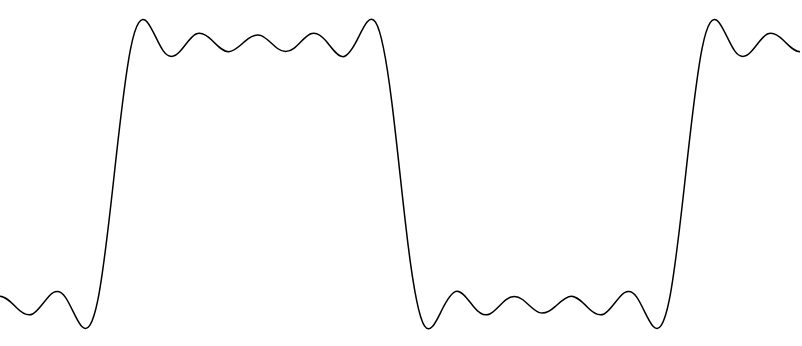
\includegraphics[width=0.6\textwidth]{Gibbs1.PNG}
    \caption{Functional approximation of square wave using 5 harmonics.}
    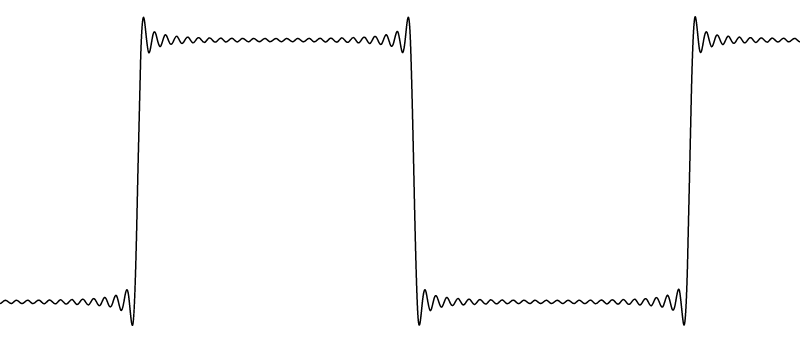
\includegraphics[width=0.6\textwidth]{Gibbs2.PNG}
    \caption{Functional approximation of square wave using 25 harmonics.}
    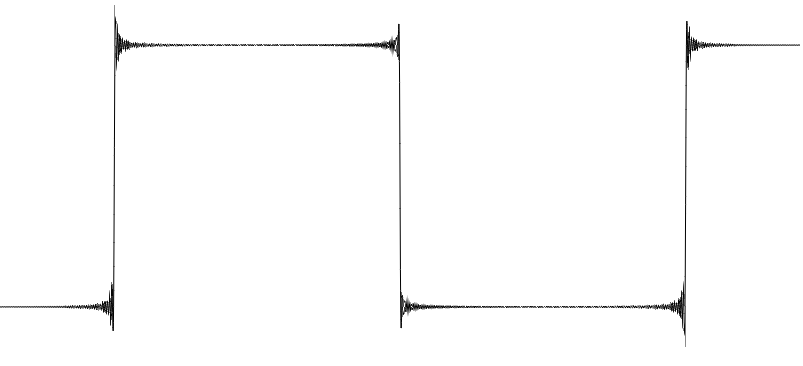
\includegraphics[width=0.6\textwidth]{Gibbs3.PNG}
    \caption{Functional approximation of square wave using 125 harmonics.}
    \label{fig:Gibbs}
\end{figure}

\par

The Gibbs phenomenon reflects the difficulty inherent in approximating a discontinuous function by a finite series of continuous sine and cosine waves. It is important to put emphasis on the word finite because even though every partial sum of the Fourier series overshoots the function it is approximating, the limit of the partial sums does not. The value of x where the maximum overshoot is achieved moves closer and closer to the discontinuity as the number of terms summed increases so, again informally, once the overshoot has passed by a particular x, convergence at that value of x is possible.


\section{The Haar System.}
\label{sec3}

\par
In mathematics, the Haar wavelet is a sequence of rescaled "square-shaped" functions which together form a wavelet family or basis. Wavelet analysis is similar to Fourier analysis in that it allows a target function over an interval to be represented in terms of an orthonormal basis. The Haar sequence is now recognized as the first known wavelet basis

\subsubsection*{The Haar Scaling Functions and the Haar Functions.}

\textbf{Definition:} Let $p(x)=X_{[0.1)}(x),$ and for each $j . k \in \mathbf{Z},$ define $p_{j . k}(x)=2^{j / 2} p\left(2^{j}, r-k\right)=D_{2}, T_{k} p(x)$. The collection $\left\{p_{j, k}(x)\right\}_{\text {t. } k \in \mathbf{Z}}$ is referred to as the system of Haar scaling function. For each $j \in \mathbf{Z}$. the collection $\left\{p_{1, k}(x)\right\}_{k \in \mathbf{Z}}$ is referred to as the system of
scale $j$ Haar scaling functions.
Let $h(x)=\chi_{[0,1 / 2)}(x)-\chi_{[1 / 2,1]}(x),$ and for each $j, k \in \mathbf{Z}$, define
$$
h_{j, k}(x)=2^{J / 2} h\left(2^{j} x-k\right)=D_{2^{j}} T_{k} h(x)
$$
The collection $\left\{h_{j, k}(x)\right\}_{j, k \in \mathbf{Z}}$ is referred to as the Haar system on $\mathbf{R}.$ For each $j \in \mathbf{Z},$ the collection $\left\{h_{J, k}(x)\right\}_{k \in \mathbf{Z}}$ is referred to as the system of scale $j$ Haar functions.


\textbf{Properties:}

\begin{itemize}
    
    \item For each $j . k \in \mathbf{Z}, p_{j . k}(x)=2^{j / 2} \mathrm{l}_{I_{j . k}}(x) .$ so that $p_{j . k}(x)$ is supported on the interval $I_{j . k}$ and does not vanish on that interval. Therefore, we refer to the scaling function $p_{j . k}(. r)$ as being associated with the interval $I_{j, k} .$
    
    \item For each $j, k \in \mathbf{Z}$
$$
\int_{\mathbf{R}} p_{j, k}(x) d x=\int_{I_{j, k}} p_{j, k}(x) d x=2^{-j / 2}
$$
and
$$
\int_{\mathbf{R}}\left|p_{j, k}(x)\right|^{2} d x=\int_{I_{j, k}}\left|p_{j, k}(x)\right|^{2} d x=1
$$
\end{itemize}

\subsection*{The Haar Bases on [0,1].}

For any integer $J \geq 0,$ the scale $J$ Haar system on $[0,1]$ is
the collection
$$
\left\{p_{J, k}(x): 0 \leq k \leq 2^{J}-1\right\} \cup\left\{h_{J, k}(x): j \geq J ; 0 \leq k \leq 2^{J}-1\right\}
$$
When $J=0,$ this collection will be referred to simply as the Haar system on $[0,1] .$

(a) The Haar system on $[0,1]$ consists of precisely those Haar functions $h_{j, k}(x)$ corresponding to dyadic intervals $I_{j, k}$ that are sub-
sets of $[0,1],$ together with the single scaling function $p_{0,0}(x)$

(b) For $J>0,$ the scale $J$ Haar system on $[0,1]$ consists of precisely those
Haar functions $h_{j, k}(x)$ corresponding to dyadic intervals $I_{j . k}$ for which $j \geq$
$J$ and that are subsets of $[0,1],$ together with those scale $J$ Haar scaling
functions that are supported in $[0,1] .$

\begin{figure}[h]
    \centering
    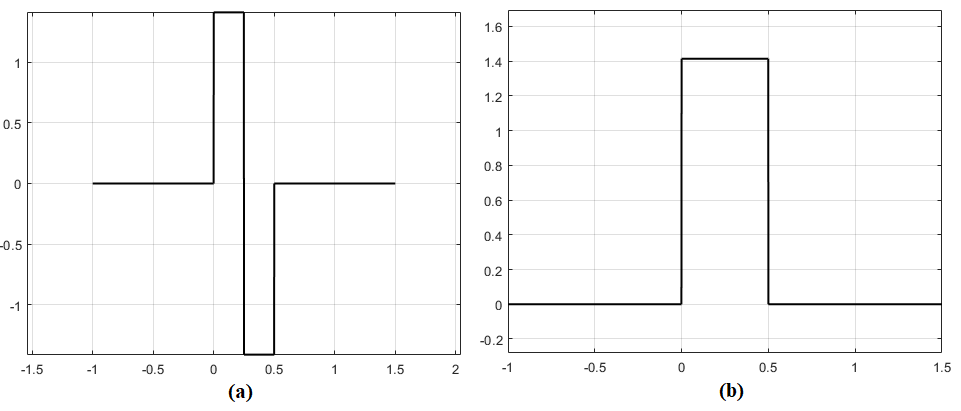
\includegraphics[width=\textwidth]{Haar_Basis.PNG}
    \caption{(a) The Haar functions $h_{\jmath, k}(x)$ on $[0,1)$, (b)Haar scaling function $p_{j, k}(x)$ on $[0,1)$.}
    \label{fig:Haar}
\end{figure}


\subsection*{Approximate and Detailed Operators.}

\par

\textbf{Definition:} For each $j \in \mathbf{Z},$ define the approximation operator $P_{j}$ on
functions $f(x), L^{2}$ on $\mathbf{R}, b y$
$$
P_{J} f(x)=\sum_{k}\left\langle f, p_{J, k}\right\rangle p_{\jmath, k}(x)
$$


(a) For each $j \in \mathbf{Z}$, define the approximation space $V_{j}$ by
$$
V_{j}=\overline{\operatorname{span}}\left\{p_{\jmath, k}(x)\right\}_{k \in \mathbf{Z}}
$$
since $\left\{p_{\jmath, k}(x): k \in \mathbf{Z}\right\}$ is an orthonormal system on $\mathbf{R} \in \mathbf{Z}$.
that $P_{j} f(x)$ is the function in $V_{j}$ best approximating $f(x)$ in the $L^{2}$ sense.

(b) since $p_{j, k}(x)=2^{j / 2} \chi_{I_{j, k}}(x)$
$$
\qquad\left(f, p_{j, k}\right) p_{j, k}(x)=\left(2^{j} \int_{I_{j, k}} f(t) d t\right) \chi_{I_{j, k}}(x) 
$$
In other words, on the interval $ I_{j, k}, P_{j} f(x)$ is the average value of $f(x)$ on ${I_{J, k}}$


\textbf{Definition:} For each $j \in \mathbf{Z},$ define the detail operator $Q_{j}$ on functions
$f(x), L^{2}$ on $\mathbf{R}, b y$
$$
Q_{j} f(x)=P_{j+1} f(x)-P_{j} f(x)
$$

\begin{figure}[h]
    \centering
    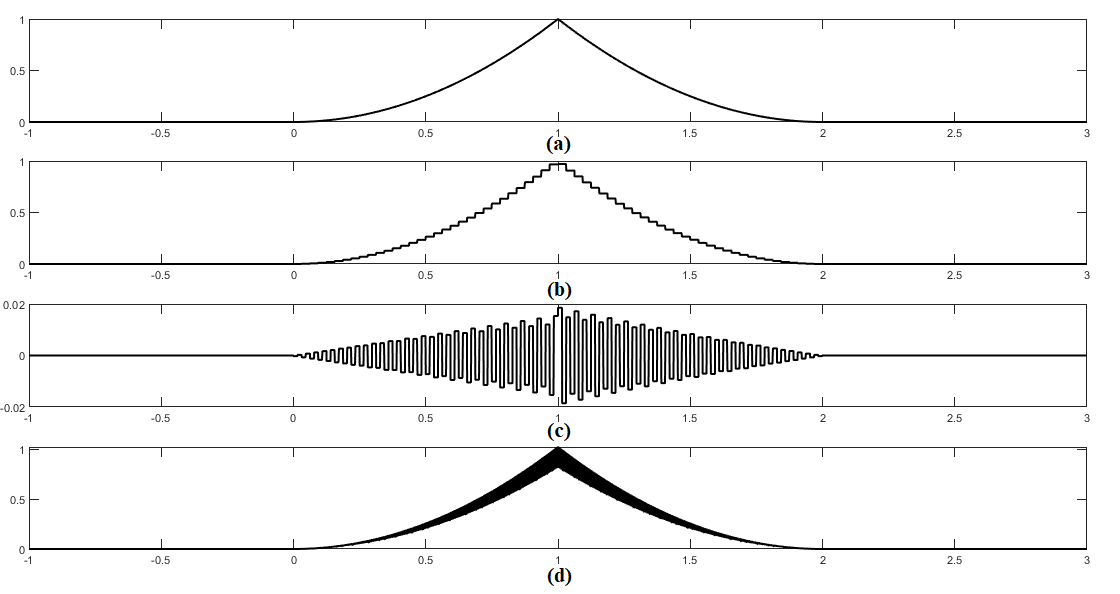
\includegraphics[width=\textwidth]{PxQxFx.png}
    \caption{(a) Approximate Operator of Second Degree Hat function, (b) Approximate Operator of Second Degree Hat function, (c) Detailed Operator of Second Degree Hat function, (d)Approximation of Second Degree Hat function Using Haar Basis.}
    \label{fig:PxQxFx}
\end{figure}


(a) For each $j \in \mathbf{Z},$ we define the wavelet space $W_{j}$ by
$$
W_{j}=\overline{\operatorname{span}}\left\{h_{J, k}(x)\right\}_{k \in \mathbf{Z}}
$$
since $\left\{h_{j, k}(x)\right\}_{k \in \mathbf{Z}}$ is an orthonormal system on $\mathbf{R}$ and in light of ( 5.12)
Lemma 2.51 implies that $Q_{j} f(x)$ is the function in $W_{j}$ best approximating
$f(x)$ in the $L^{2}$ sense.

(b) In light of the interpretation of $P_{j} f(x)$ as the blurred version of $f(x)$
at scale $2^{-j},$ we can interpret $Q_{j} f(x)$ as containing those features of $f(x)$
that are of size smaller than $2^{-J}$ but larger than $2^{-\jmath-1} .$ That is, $Q_{j} f(x)$
has those details invisible to the approximation $P_{j} f(x)$ but visible to the
approximation $P_{J+1} f(x)$

\section{The Discrete Haar Transform in 1 Dimension.}

\subsection*{Motivation.}
\par

A function $f(x)$ (defined on [ 0.1] his an expansion in terms of
Haar functions as follows. Give that any integer $J \geq 0$.
$$
f(x)=\sum_{j=J}^{x} \sum_{k=0}^{2^{\prime}-1}\left\langle f \cdot h_{j \cdot k}\right\rangle h_{J, k} \cdot(x)+\sum_{k=0}^{2^{\prime}-1}\left\langle f \cdot p_{J, k}\right\rangle p_{J, k}(x)
$$

in $L^{2}$ on $[0.1]$

Thus. the Haar coefficients of $f(x)$ can be approximated by the Haar coefficients of $P_{N} f(x)$. That is.
$$
\left\langle f . h_{J . k}\right\rangle \approx\left\langle P_{N} f . h_{J . k}\right\rangle \quad \text { and } \quad\left\langle f, p_{J . k}\right\rangle \approx\left\langle P_{N} f, p_{J . k}\right\rangle
$$

\subsection*{Derivation.}
\par

Suppose that we are given a finite sequence of data of length $2^{N}$ for some
$N \in \mathbf{N} .\left\{c_{0}(k)\right\}_{k=0}^{2}-1$. We assume that for some underlying function $f(x)$
$c_{0}(k)=\left\langle f \cdot p_{N, k}\right\rangle .$ Fix $J \in \mathbf{N} . J<N .$ and for each $1 \leq j \leq J,$ define,

$c_{j}(k)=\left\langle f, p_{N-j, k}\right\rangle \quad$ and $\quad d_{j}(k)=\left\langle f . h_{N-j . .\rangle}\right\rangle$

\par
It turns out that there is a convenient recursive algorithm that can be used to compute the coefficients $c_{j}(k)$ and $d_{j}(k)$ from $c_{j-1}(k) .$.

$\begin{aligned} c_{j}(k) &=\left\langle f, p_{N}-, . k\right\rangle \\ &=\frac{1}{\sqrt{2}}\left\langle f, p_{N}-j+1.2 k\right\rangle+\frac{1}{\sqrt{2}}\left\langle f \cdot p_{N}-j+1,2 k+1\right\rangle \\ &=\frac{1}{\sqrt{2}} c_{J-1}(2 k)+\frac{1}{\sqrt{2}} c_{J-1}(2 k+1) \\ &=\frac{1}{\sqrt{2}} c_{j-1}(2 k)-\frac{1}{\sqrt{2}} c_{j-1}(2 k+1) \end{aligned}$

$d_{j}(k)=\frac{1}{\sqrt{2}} c_{j-1}(2 k)-\frac{1}{\sqrt{2}} c_{j-1}(2 k+1)$

By writing in Matrix form,
$$
\left(\begin{array}{c}{c_{j}(k)} \\ {d_{j}(k)}\end{array}\right)=\frac{1}{\sqrt{2}}\left(\begin{array}{cc}{1} & {1} \\ {1} & {-1}\end{array}\right)\left(\begin{array}{c}{c_{j-1}\left(2 k_{i}\right)} \\ {c_{j-1}(2 k+1)}\end{array}\right)
$$

$$
\left(\begin{array}{c}{c_{j-1}(2 k)} \\ {\left(\cdot_{j-1}(2 k+1)\right.}\end{array}\right)=\frac{1}{\sqrt{2}}\left(\begin{array}{cc}{1} & {1} \\ {1} & {-1}\end{array}\right)\left(\begin{array}{c}{c_{j}(k)} \\ {d_{j}(k)}\end{array}\right)
$$

As with the DFT, the DHT can be thought of as a linear transformation on a finite-dimensional space and as such can be written as multiplication by a matrix.

Given $L \in \mathbf{N}$ even, define the $(L / 2) \times L$ matrices $H_{L}$ and $G_{L}$ by:

$$
H_{L}=\frac{1}{\sqrt{2}}\left(\begin{array}{cccccc}{1} & {1} & {0} & {} & {\cdots} & {0} \\ {0} & {0} & {1} & {1} & {0} & {\cdots} & {0} \\ {} & {} & {} & {\vdots} & {} \\ {0} & {} & {\cdots} & {} & {0} & {1} & {1}\end{array}\right)
$$

$$
G_{L}=\frac{1}{\sqrt{2}}\left(\begin{array}{cccccc}{1} & {-1} & {0} & {} & {\cdots} & {0} \\ {0} & {0} & {1} & {-1} & {0} & {\cdots} & {0} \\ {} & {} & {} & {\vdots} \\ {0} & {} & {\cdots} & {} & {0} & {1} & {-1}\end{array}\right)
$$

Define the $L \times L$ matrix $\mathcal{W}_{L}$ by
$$
\mathcal{W}_{L}=\left(\begin{array}{c}{H_{L}} \\ {G_{L}}\end{array}\right)
$$
The matrix $H_{L}$ is referred to as the approximation matrix, the matrix $G_{L}$ as the detail matrix, and the matrix $\mathcal{W}_{L}$ as the wavelet matrix.

\subsection*{Algorithms for DHT and IDHT}

\textbf{Discrete Haar Transform:} Given $J, N \in \mathbf{N}$ with $J<N$ and a vector
$$
\mathbf{c}_{0}=\left(c_{0}(0) c_{0}(1) \cdots c_{0}\left(2^{N}-1\right)\right)
$$
of length $2^{N},$ the $D H T$ of $\mathbf{c}_{0}$ is the vector
$$
\left(\begin{array}{ll}{d_{1}} & {d_{2}}\end{array} \cdots d_{J} c_{J}\right)
$$
where,
$$
\left(\begin{array}{c}{\mathbf{c}_{J}} \\ {\mathbf{d}_{j}}\end{array}\right)=\left(\begin{array}{c}{H} \\ {G}\end{array}\right) \mathbf{c}_{\jmath-1}
$$

\begin{figure}[h]
    \centering
    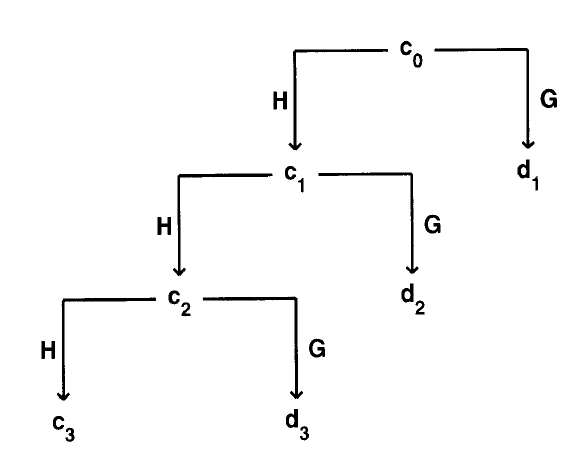
\includegraphics[width=0.5\textwidth]{Tree.PNG}
    \caption{Tree Diagram for The DHT.}
    \label{fig:DHTS}
\end{figure}

\subsection{ Comparison of Discrete Haar Wavelet Transform with Discrete Cosine Transform.}
\par
As shown in the figure,the lossy compression is performed on the given discrete signal by using discrete Haar transform (DHT) and by using discrete cosine transform (DCT).   

\begin{figure}[h]
    \centering
    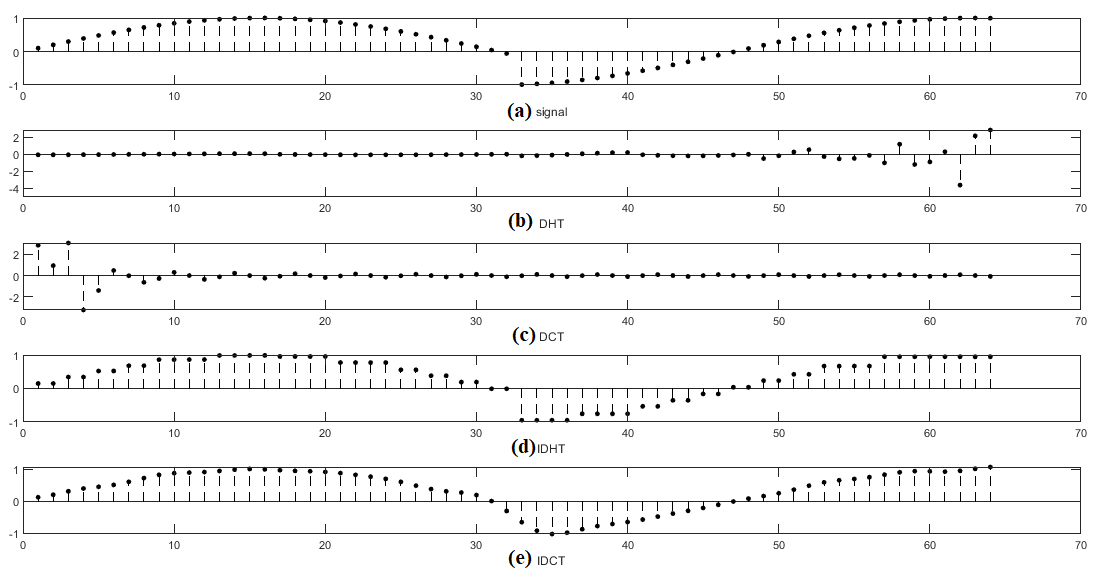
\includegraphics[width=\textwidth]{dht.png}
    \caption{(a) Original Discrete Signal, (b) DHT of the Signal, (c) DCT of the Signal,(d) IDHT of Compressed Signal, (e) IDCT of Compressed Signal.}
    \label{fig:dht_dct}
\end{figure}

As we can see, the information at the discontinuity in the original signal is sustained by the DHT method whereas, it is smoothed out in the case of DCT method.  

\section{The Discrete Haar Transform in 2 Dimensions.}
\label{sec5}

In many applications, especially image processing, the objects being analyzed are best thought of as matrices, rather than one-dimensional finite signals. That is, we are interested in $L \times M$ matrices $c$ of the form $c=\{c(n, m): 0 \leq n \leq L-1 ; 0 \leq m \leq M-1\} .$ The purpose of this section is to define a generalization of the DHT for matrices.

Given an even number $L \in \mathbf{N},$ let $H$ and $G$ be the $(L / 2) \times L$ matrices. Let $c$ be an $M \times L$ matrix of the form
$$
c=\left(\begin{array}{c}{c_{0}} \\ {c_{1}} \\ {\cdots} \\ {c_{M-1}}\end{array}\right)
$$

In this notation, $c_{\ell}$ is the $\ell$ th row of $c .$ We define the row-wise approximation matrix of $c, \mathbf{H}^{\text {row }} c,$ to be the $M \times(L / 2)$ matrix defined by
$$
\mathbf{H}^{\text {row }} c=\left(\begin{array}{c}{H c_{0}} \\ {\text { He}_{1}} \\ {\cdots} \\ {H c_{M-1}}\end{array}\right)
$$

We define the row-wise detail matrix of $c,$ Grow $c, |$ to be the $M \times(L / 2)$
matrix defined by:
$$
\mathbf{G}^{\text {row }} c=\left(\begin{array}{c}{G c_{0}} \\ {G c_{1}} \\ {\cdots} \\ {G c_{M-1}}\end{array}\right)
$$


Given $L \in \mathbf{N}$ even, let $c$ be an $L \times M$ matrix of the form
$$
c=\left(\begin{array}{cccc}{c_{0}} & {c_{1}} & {\cdots} & {c_{M-1}}\end{array}\right)
$$
where $c_{\ell}$ is the $\ell^{t h}$ column of $c$. We define the column-wise approximation matrix of $c, \mathbf{H}^{\operatorname{col}} c,$ to be the $(L / 2) \times M$ matrix defined by
$$
\mathbf{H}^{\operatorname{col}} c=\left(\begin{array}{cccc}{H c_{0}} & {H c_{1}} & {\cdots} & {H c_{M-1}}\end{array}\right)
$$

We define the column-wise detail matrix of $c, \mathrm{G}^{\mathrm{rOW}} c,$ to be the $(L / 2) \times M$ matrix defined by
$$
\mathrm{G}^{\mathrm{col}} c=\left(\begin{array}{cccc}{G c_{0}} & {G c_{1}} & {\cdots} & {G c_{M-1}}\end{array}\right)
$$

\subsection{The DHT for the Matrices.}

Given J, $N \in \mathbf{N}$ with $J<N$ and a matrix $c_{0}=\{c(n, m)\}_{n, m=0}^{N-1}$
For $1 \leq j \leq J,$ define the 2 $^{N-3} \times 2^{N-j}$ matrices $c_{j} d_{j}^{(1)}, d_{j}^{(2)},$ and $d_{j}^{(3)}$ by
$$
\begin{aligned} c_{j} &=\mathbf{H}^{\text {col }} \mathbf{H}^{\text {row }} c_{j-1} \\ d_{j}^{(1)} &=\mathbf{G}^{\text {col }} \mathbf{H}^{\text {row }} c_{j-1} \\ d_{j}^{(2)} &=\mathbf{H}^{\text {col }} \mathbf{G}^{\text {row }} c_{j-1} \\ d_{j}^{(3)} &=\mathbf{G}^{\text {col }} \mathbf{G}^{\text {row }} c_{j-1} \end{aligned}
$$

where $\mathbf{H}^{\mathrm{col}}, \mathbf{G}^{\mathrm{col}}, \mathbf{H}^{\mathrm{row}},$ and $\mathbf{G}^{\mathrm{row}}$ are the $2^{N-j-2} \times 2^{N-j-1}$. The $D H T$ of $c_{0}$ is the collection of matrices
$$
\left\{d_{j}^{(1)}, d_{j}^{(2)}, d_{j}^{(3)}\right\}_{j=1}^{J} \cup\left\{c_{J}\right\}
$$


\subsection{The IDHT for the Matrices.}

Given $L \in \mathbb{N}$, let $H^{*}$ alld $G^{*}$ loc the adjoints of $H$ and $G$. Let $c$ be
all $M \times(L / 2)$ matrix of the form,
$$
c=\left(\begin{array}{c}{c_{1}} \\ {c_{1}} \\ {\cdots} \\ {c_{M-1}}\end{array}\right)
$$
We define the row-wise approximation adjoint of $r . \mathbf{H}^{\mathrm{rOW}^{*}} c$. to be the $M \times L$ Matrix.

$$
\mathbf{H}^{\mathrm{row} *} c=\left(\begin{array}{c}{H^{*} c_{0}} \\ {H^{*} c_{1}} \\ {\cdots} \\ {H^{*}(n /-1)}\end{array}\right)
$$

We define the row-wise detail adjoint of $C . \mathrm{G}^{\mathrm{row} *}$ c. to be the $M \times L$ matrix
$$
\mathrm{G}^{\mathrm{row}^{*}} c=\left(\begin{array}{c}{G^{*} c_{0}} \\ {G^{*} c_{1}} \\ {\cdots} \\ {G^{*} c_{M-1}}\end{array}\right)
$$

${H_{row}}^{c}$ is the matrix obtained by multiplying each row of $c$ by the matrix
$H^{*},$ and $\mathrm{G}^{\mathrm{row}^{*}} c$ is the matrix obtained by multiplying each row of $c$ by the matrix $G^{*}$. Given $L \in \mathbb{N}$ even, let $c$ be an $(L / 2) \times M$ matrix of the form
$$
c=\left(\begin{array}{cccc}{c_{0}} & {c_{1}} & {\cdots} & {c_{M-1}}\end{array}\right)
$$
We define the column wise approximation adjoint of $c . \mathbf{H}^{\mathrm{col}^{*}} c .$ to be this $L \times M$ matrix,

$$
\mathbf{H}^{\mathrm{COl}^{*}} c=\left(\begin{array}{cccc}{H^{*} c_{0}} & {H^{*} c_{1}} & {\cdots} & {H^{*} c_{M-1}}\end{array}\right)
$$
We define the column-wise detail adjoint of $c .$ Grow $_{C} .$ to be the $L \times M$
matrix
$$
\mathbf{G}^{\mathrm{col}^{*}} c=\left(\begin{array}{cccc}{G^{*} c_{0}} & {G^{*} c_{1}} & {\cdots} & {G^{*} c_{M-1}^{*}}\end{array}\right)
$$

The inverse $D H T$ for matrices is given by
$$
\begin{aligned} c_{3-1}=\mathbf{H}^{\mathrm{row}^{*}} \mathbf{H}^{\mathrm{col}^{*}} c_{3}+\mathbf{H}^{\mathrm{row}^{*}} \mathbf{G}^{\mathrm{col}^{*}} d_{j}^{(1)} \\ &+\mathbf{G}^{\mathrm{row}^{*}} \mathbf{H}^{\mathrm{col}^{*}} d_{3}^{(2)}+\mathbf{G}^{\mathrm{row}^{*}} \mathbf{G}^{\mathrm{col}^{*}} d_{j}^{(3)} \end{aligned}
$$
where $\mathbf{H}^{\mathrm{col}}, \mathbf{G}^{\mathrm{col}}, \mathbf{H}^{\mathrm{row}},$ and $\mathbf{G}^{\mathrm{row}}$ are $2^{N-3-2} \times 2^{N-3-1}$ matrices given above.


\section{Image Compression Using Discrete Haar Wavelet Transform.}
\label{sec6}

\par 
As shown in the figure below, the Discrete Haar Wavelet Transform and The Discrete Cosine Transforms are taken. As most of the pixel values are near to the zero (i.e. black), image can be compressed by setting those values to zero.  

\begin{figure}[h]
    \centering
    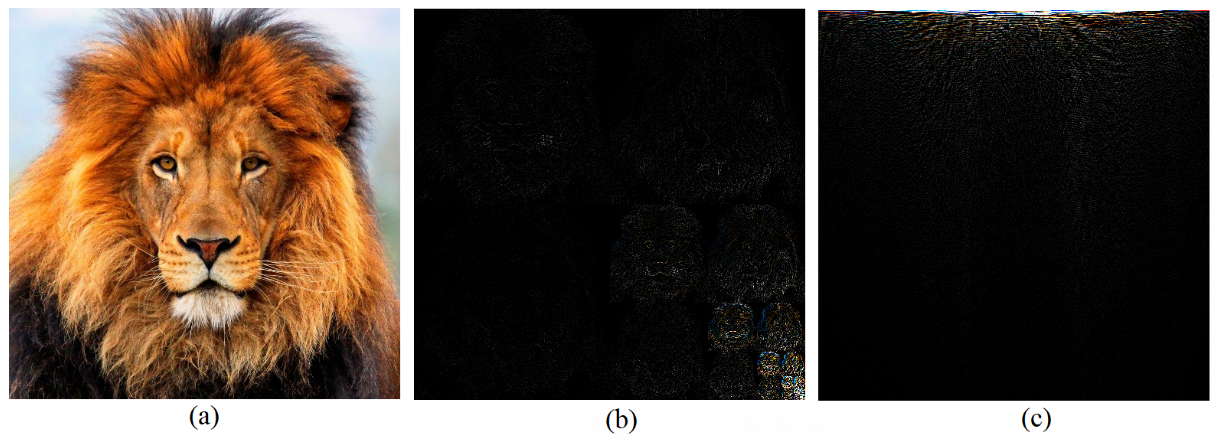
\includegraphics[width=\textwidth]{LionDCTDHT.PNG}
    \caption{(a) Original Image, (b) DHT of the Image, (c) DCT of the Image.}
    \label{fig:imgdctdht}
\end{figure}

Hence, by applying lossy compression on the Discrete Cosine Transform of the image, The Inverse Discrete Cosine Transform of the compressed images are given by:

\begin{figure}[h]
    \centering
    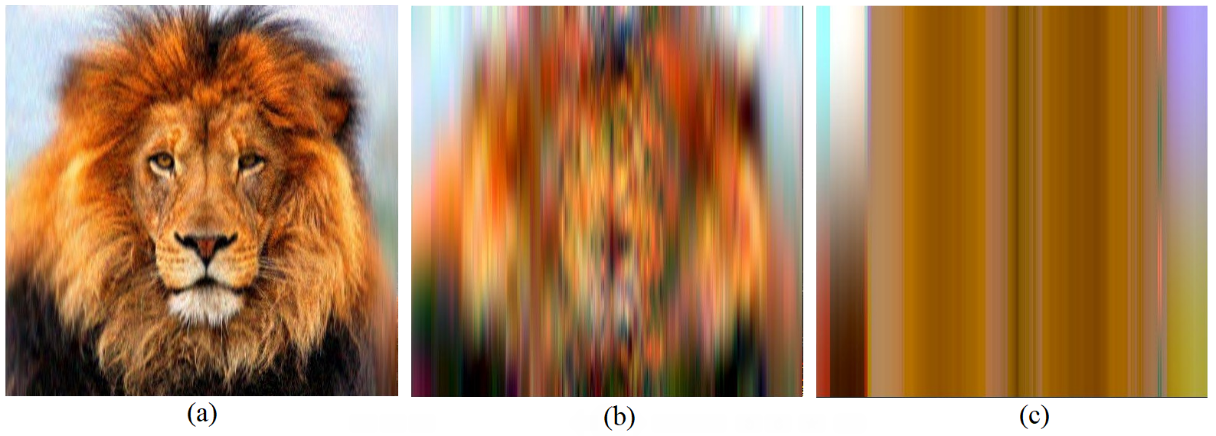
\includegraphics[width=\textwidth]{LionDCTcmp.PNG}
    \caption{(a) 97\% compressed using DCT, (b) 99\% compressed using DCT, (c) 99.99\% compressed using DCT.}
    \label{fig:imgdct}
\end{figure}

Similarly, applying lossy compression on the Discrete Haar Transform of the image, The Inverse Discrete Haar Transform of the compressed images are given by:


\begin{figure}[h]
    \centering
    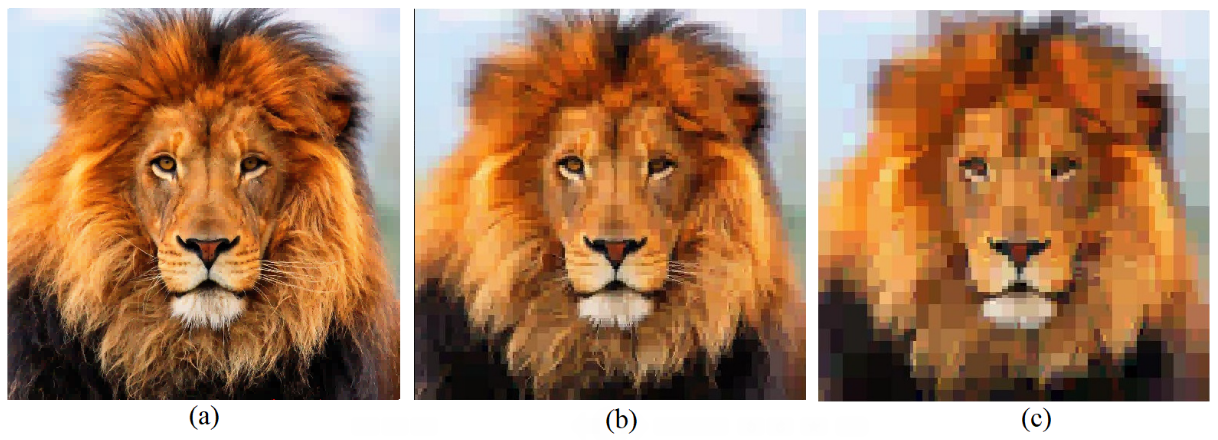
\includegraphics[width=\textwidth]{LionDHTcmp.PNG}
    \caption{(a) 97\% compressed using DHT, (b) 99\% compressed using DHT, (c) 99.99\% compressed using DHT.}
    \label{fig:imgdht}
\end{figure}

\section{Conclusions.}

The normalized version of the Haar wavelet offers greater compression, and yields better-looking results compared to the standard one. This is due to the properties of orthogonal matrices. The variant that implements loops to perform the normalization in the Haar wavelet transformation process is better in terms of algorithm complexity compared to the variant that generates the required Haar matrices and performs matrix multiplication. Throughout this project, we focused on the Haar wavelet transform as a window to better understanding the different compression processes since they boil down to the same essence. Thus, this research and implementation have been useful in terms of gaining a lot of insight into the field of image compression and its application of mathematical concepts 

\section{REFERENCES}

\begin{enumerate}
    \item[[ 1]]   Walnut, David $\mathrm{F}$. An introduction to wavelet analysis / David F. Walnut p. cm. (Applied and numerical harmonic analysis) Includes bibliographical references and index. ISBN $0-8176-3962-4$ (alk. paper).
    \item[[ 2]]  Stéphane Mallat, a Wavelet tour of signal processing,The Sparse Way,ISBN $13: 9780-12-374370-1$.
    \item[[ 3]] A. Haar. Zur theorie der orthogonalen funktionensysteme. Math. Annal., 69:331–371, 1910.
\end{enumerate}





